\documentclass{article}

\usepackage{fancyhdr, ragged2e, indentfirst, longtable, tabu, graphicx, float, hhline, makecell, bookmark}
\usepackage[table]{xcolor}
\usepackage[letterpaper, total={7in, 9in}]{geometry}

\graphicspath{ {./imgs/} }

\makeatletter
\title{Documento de Arquitectura del Software} \let\Title\@title
\date{Septiembre 2018} \let\Date\@date
\author{Valentina Hernández} \let\Author\@author
\makeatother

\pagestyle{fancy}
\fancyhf{}
\rhead{Versión: 1.0 \\ \Date}
\lhead{CPI \\ DAS \\ Identificador del documento}

\lfoot{Confidencial}
\cfoot{iKels Consulting \\ \Date}
\rfoot{Pag. \thepage}

\renewcommand{\headrulewidth}{1pt}
\renewcommand{\footrulewidth}{1pt}
\renewcommand{\contentsname}{Índice}

\newcommand\Tstrut{\rule{0pt}{2.6ex}}       % "top" strut
\newcommand\Bstrut{\rule[-0.9ex]{0pt}{0pt}} % "bottom" strut
\newcommand{\TBstrut}{\Tstrut\Bstrut}       % top&bottom struts

\renewcommand{\cellalign}{cl}
\renewcommand\cellgape{\gape[t]}

\begin{document}

    \newgeometry{textwidth=12cm,textheight=10cm}
    \begin{titlepage}
        \huge{\Title}
        \begin{flushright}
            \Large{CPI \\ Versión: 1.0}
        \end{flushright}
    \end{titlepage}

    \restoregeometry

    \newpage
    \tableofcontents

    \newpage
    \begin{center}
        \begin{tabular}{ |c|c|c|c| }
            \hline
            \rowcolor{blue!25}
            Fecha & Versión & Descripción & Autores \\ [0.5ex]
            \hline\hline
            29/09/2018 & 1.0 & Documento de Arquitectura & Valentina Hernández \\
            \hline
        \end{tabular}
    \end{center}

    \newpage
    \section{Introducción}
    \subsection{Propósito}
    Este documento permitirá a los involucrados en el desarrollo de este sistema, tener una visión general de su arquitectura. Sirviendo como guía para el desarrollo, la identificación de las funcionalidades al dar una visión detallada de ellas, así como para dar una base informativa para el mantenimiento del sistema por parte del equipo de trabajo original o de terceros.

    \subsection{Alcance}
    A continuación se presenta una abstracción de la estructura que debe tener el sistema, el presente documento servirá de guía para los desarrolladores, usuarios y stakeholders para conocer los requerimientos del sistema, el diseño de la base de datos, así como mostrar sus funcionalidades y como están implementadas en el sistema. 
 
    Esta información es importante para dar una explicación clara de cómo está diseñado el sistema y así facilitar la mantenibilidad del mismo.

    \subsection{Definiciones, Siglas y Abreviaciones}

    \subsection{Referencias}
    No hace referencia a ningún otro documento.

    \subsection{Vista Global}
    Este documento contiene todas las especificaciones de la arquitectura de la aplicación web \emph{CPI} tanto a nivel de hardware como de software. Se introduce la representación arquitectónica del sistema, especificando en detalle los objetivos y restricciones de la misma, los casos de uso, procesos dentro del sistema, la implantación, implementación, los datos almacenados, tamaño, desempeño y calidad. También se explicará datos importantes del sistema mediante diagramas de actividades, de casos de uso, de clases, diagrama ERE, etc.

    \vskip 1.5cm
    \section{Representación Arquitectónica} \label{reprArq}
    La representación arquitectónica de \emph{CPI} está basada en el modelo de 4+1 vistas de Philippe Kruchten. En el transcurso del documento se tratarán más a fondo los detalles de cada una.
    
    
    \section{Vista Lógica} \label{vistaLogica}
    \subsection{Vista General}
    \subsubsection{Diagrama Conceptual (Modelo de Dominio)}
    \subsubsection{Diagrama de Clases}
    
\pagebreak
\section{Vista de Desarrollo} \label{vistaImplementacion}
La Vista de Desarrollo de la aplicación se hizo a través de un diagrama de componentes, en donde se especifica la relación entre los mismos. Se tomaron en cuenta los componentes principales de la aplicación para facilitar al lector la comprensión del mismo.
A continuación se muestra el Diagrama de componentes en la Figura \ref{fig:diagrama_componentes}.

\begin{figure}[H]
   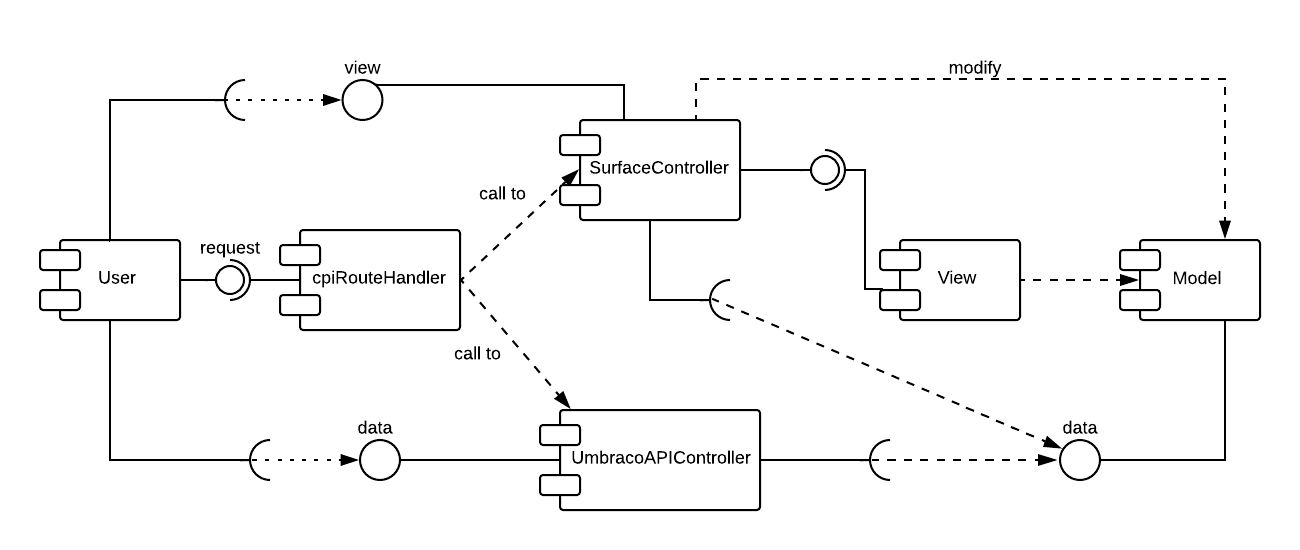
\includegraphics[width=\textwidth]{diagrama_componentes.png}
   \caption{Diagrama de Componentes. Elaboración propia.}
   \label{fig:diagrama_componentes}
   \centering
\end{figure}
    \vskip 2cm

\section{Vista de Procesos} \label{vistaProcesos}
En esta vista se muestran tanto los aspectos concurrentes del sistema a tiempo de ejecución como las interacciones que ocurren entre ellos. Sin embargo esta vista no fue desarrollada dado que la aplicación no resuelve aspectos de concurrencia de usuarios ni de datos.


    \vskip 1.5cm
\section{Vista Física} \label{vistaFisica}
La Vista Física muestra las plataformas de hardware y software necesarias para la ejecución del sistema. Esta vista se ve reflejada en la Figura \ref{fig:diagrama_despliegue}.

En el diagrama se puede apreciar la disposición física de los componentes del software, partiendo desde el equipo del usuario representante de la cadena, los usuarios ingresan al Sistema por medio de un navegador Web en cualquier equipo de cómputo que tenga acceso a Internet. Dicho Sistema se encuentra alojado en un servidor web. Para cada petición de datos se accede al servidor de base de datos, el cual contiene la base datos de la aplicación.

\begin{figure}[H]
   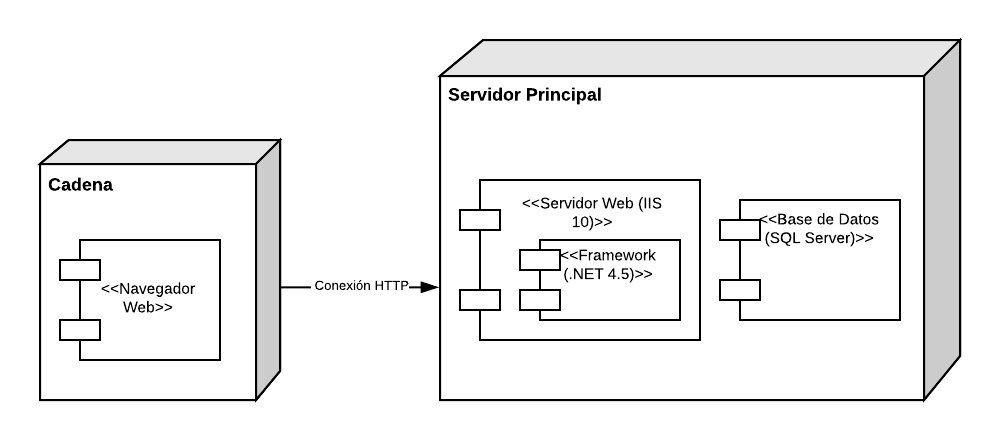
\includegraphics[width=\textwidth]{diagrama_despliegue.png}
   \caption{Diagrama de Despliegue. Elaboración propia.}
   \label{fig:diagrama_despliegue}
   \centering
\end{figure}
    \vskip 2cm
    \section{Vista de Casos de Uso} \label{vistaCasosDeUso}
    En esta vista se describirá el sistema desde el punto de vista de los casos de uso. El sistema tiene 2 actores principales:

    \begin{itemize}
        \item \emph{Admin}: Administrador de CPI. Es un usuario de Umbraco, lo que quiere decir que cuenta con las credenciales para poder ingresar al back-end de Umbraco y tiene los permisos necesarios para administrar las entidades y los grupos de CPI.
        \item \emph{Retailer}: Representa a una cadena. Solo tiene acceso a la información referente a las tiendas y productos que pertenecen a la cadena.
    \end{itemize}
    En el back office de Umbraco en la sección Member, se creó un grupo llamado \emph{cpi-user} en el que los miembros pertenientes al mismo, tienen las credenciales necesarias para acceder al sistema CPI.
    
\pagebreak
    \subsection{Resumen de Casos de Uso}
    \newcounter{magicrownumbers}
    \newcommand\rownumber{\stepcounter{magicrownumbers}\arabic{magicrownumbers}}
    \begin{center}
        \begin{longtable}{ | l | l | c | }
            \hline
            \rowcolor{blue!25}
            \multicolumn{1}{|c|}{ID del Caso de Uso} &
            \multicolumn{1}{|c|}{Caso de Uso} &
            \multicolumn{1}{|c|}{Actor} \\
            \hhline{===}
            \endhead

            \endfoot

           CU-\rownumber & Iniciar sesión (Umbraco) & Admin \\ \hline
           CU-\rownumber & Consultar lista miembros & Admin \\ \hline
           CU-\rownumber & Gestionar miembro (CRUD) & Admin \\ \hline
           CU-\rownumber & Consultar grupos & Admin \\ \hline
           CU-\rownumber & Gestionar grupo (CRUD) & Admin \\ \hline
           CU-\rownumber & Asignar miembro/s a grupo & Admin \\ \hline
           CU-\rownumber & Remover miembro/s de grupo (CRUD) & Admin \\ \hline
           CU-\rownumber & Cambiar permisos de miembro & Admin \\ \hline

           CU-\rownumber & Gestionar contenido & Admin \\ \hline
           CU-\rownumber & Consultar lista de cadenas & Admin \\ \hline
           CU-\rownumber & Gestionar cadena (CRUD) & Admin \\ \hline
           CU-\rownumber & Consultar lista de productos & Admin \\ \hline
           CU-\rownumber & Gestionar producto (CRUD) & Admin \\ \hline
           CU-\rownumber & Consultar lista de productos UPC & Admin \\ \hline
           CU-\rownumber & Gestionar producto UPC (CRUD) & Admin \\ \hline
           CU-\rownumber & Asignar producto/s a producto UPC & Admin \\ \hline
           CU-\rownumber & Remover producto/s de producto UPC & Admin \\ \hline
           CU-\rownumber & Consultar lista de precios & Admin \\ \hline
           CU-\rownumber & Consultar lista de tiendas & Admin \\ \hline
           CU-\rownumber & Gestionar tienda (CRUD) & Admin \\ \hline
           CU-\rownumber & Asignar tienda a cadena & Admin \\ \hline
           CU-\rownumber & Consultar lista de zonas & Admin \\ \hline
           CU-\rownumber & Gestionar zonas (CRUD) & Admin \\ \hline
	       CU-\rownumber & Consultar lista de catálogo generales & Admin \\ \hline
           CU-\rownumber & Gestionar catálogo (CRUD) & Admin \\ \hline
           CU-\rownumber & Asignar producto/s a catálogo & Admin \\ \hline
           CU-\rownumber & Remover producto/s de catálogo & Admin \\ \hline

           
           CU-\rownumber & Iniciar sesión (CPI) & Retailer \\ \hline
           CU-\rownumber & Consultar lista de productos & Retailer \\ \hline
           CU-\rownumber & Importar precios desde archivo excel & Retailer \\ \hline
           CU-\rownumber & Consultar reporte precio producto & Retailer \\ \hline
           CU-\rownumber & Exportar reporte precio producto & Retailer \\ \hline
           CU-\rownumber & Filtrar reporte precio producto por fecha & Retailer \\ \hline
           CU-\rownumber & Consultar reporte precio histórico de producto & Retailer \\ \hline
           CU-\rownumber & Filtrar reporte precio histórico por fechas & Retailer \\ \hline
           CU-\rownumber & Consultar reporte gráfico dispersión por catálogo & Retailer \\ \hline
           CU-\rownumber & Exportar reporte gráfico dispersión por catálogo & Retailer \\ \hline
           CU-\rownumber & Filtrar gráfico dispersión por catálogo & Retailer \\ \hline
           CU-\rownumber & Filtrar gráfico dispersión por fecha & Retailer \\ \hline
           CU-\rownumber & Consultar lista de catálogos personalizados & Retailer \\ \hline
           CU-\rownumber & Gestionar catálogo (CRUD) & Retailer \\ \hline
           CU-\rownumber & Asignar producto/s a catálogo & Retailer \\ \hline
           CU-\rownumber & Remover producto/s de catálogo & Retailer \\ \hline

        \end{longtable}
    \end{center}
\pagebreak
    \subsection{Diagrama de Casos de Uso}
    Se separaron los casos de uso en varios diagramas para facilitar la lectura.

    \begin{figure}[H]
        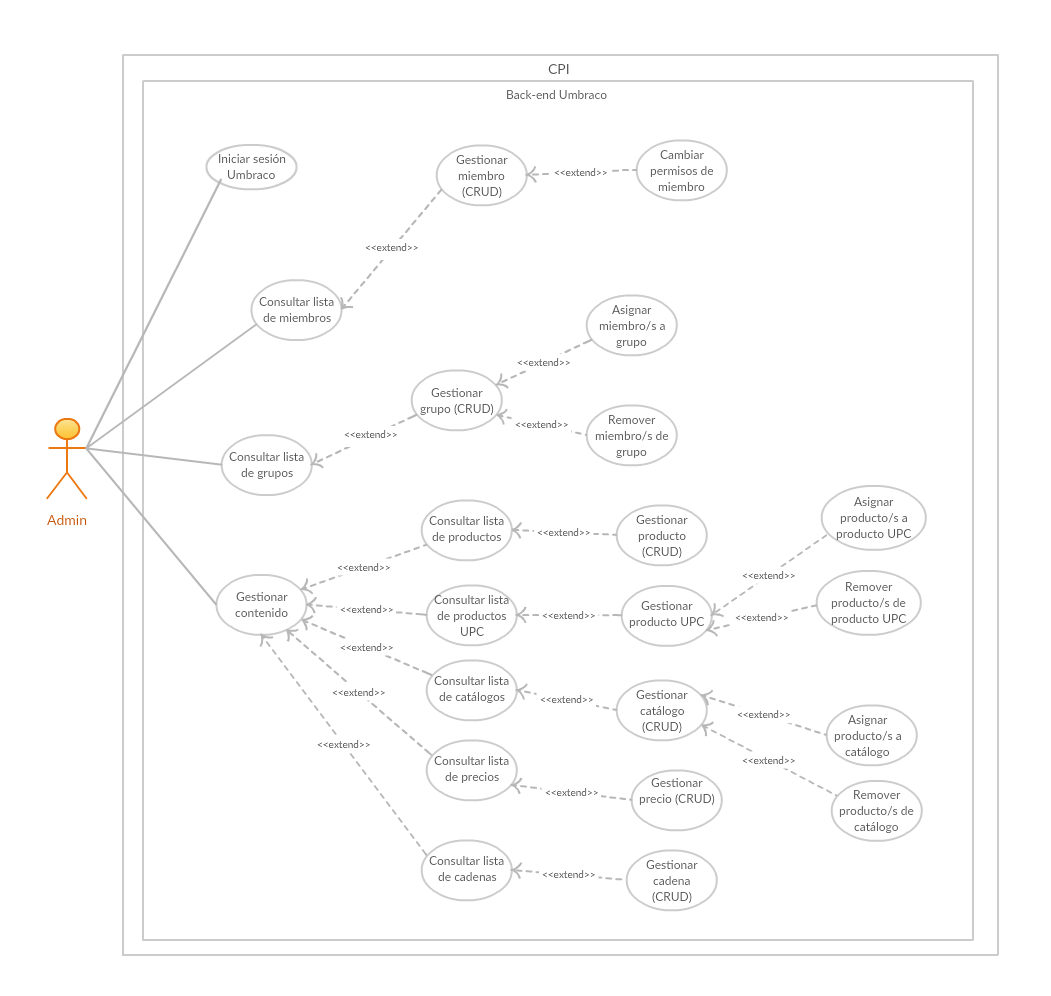
\includegraphics[width=\textwidth]{cu_admin.png}
        \caption{Casos de uso para usuario Admin}
        \label{fig:cu_admin}
        \centering
    \end{figure}

    \begin{figure}[H]
        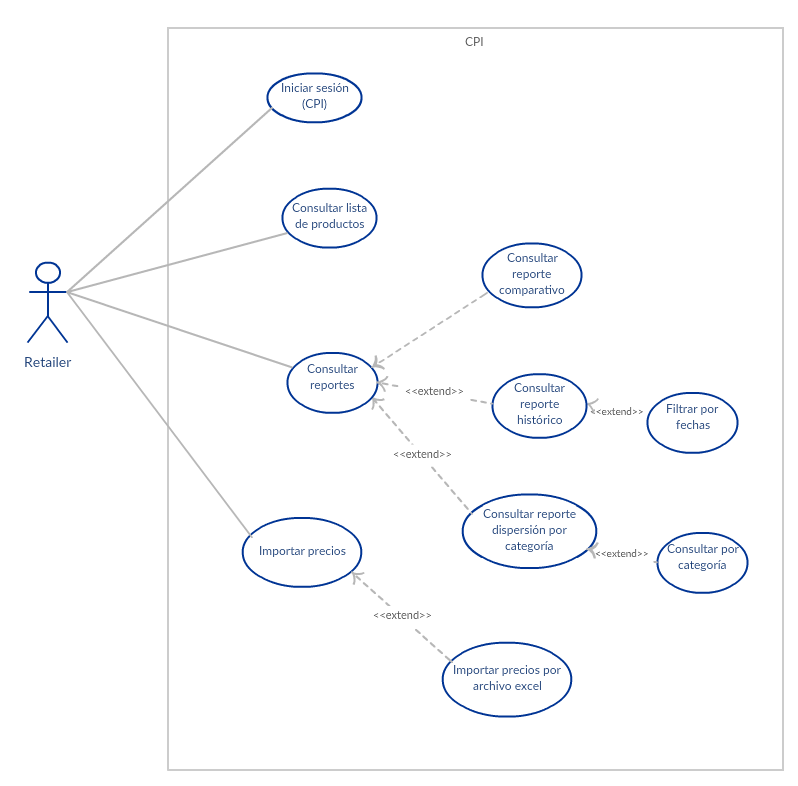
\includegraphics[scale=0.8]{cu_retailer.png}
        \caption{Casos de uso para usuario Retailer}
        \label{fig:cu_retailer}
        \centering
    \end{figure}
\pagebreak
    \subsection{Especificaciones de Casos de Uso}
    A continuación las narrativas de los casos de uso:

    \begin{center}
        \begin{longtabu} to 0.9\textwidth { | X[p] | X[p] | }
            \hline
            \multicolumn{2}{|l|}{
                \cellcolor{blue!25}{\large{\textbf{Caso de Uso:}} Iniciar sesión (Umbraco)}
            } \TBstrut \\
            \hline\hline

            \multicolumn{2}{|l|}{
                \makecell{\large{\textbf{Descripción:}} \\ El usuario quiere ingresar al back end de Umbraco.}
            } \\
            \hline

            \multicolumn{2}{|l|}{
                \makecell{\large{\textbf{Precondición:}} \\ Ingresar la dirección correcta del sitio en la barra de navegación.}
            } \\
            \hline


            \multicolumn{2}{|l|}{\cellcolor{blue!15}\large{\textbf{Flujo básico:}}}  \TBstrut\\
            \hline

            Actor & Sistema \TBstrut\\
            \hline
            1. El actor abre su navegador e introduce la dirección correspondiente al back end de Umbraco. &  \\ [0.3ex]
            \hline
             & 2. El servidor procesa la solicitud y envía al navegador del cliente una ventana para que el usuario se autentique. \\ [0.3ex]
             \hline
             3. El actor introduce su email y su contraseña. &  \\ [0.3ex]
             \hline
             & 4. El sistema valida la información del usuario y lo redirige al tablero (back end) de Umbraco. \\ [0.3ex]
             \hline\hline


            \multicolumn{2}{|l|}{\cellcolor{blue!15}\large{\textbf{Flujos alternos:}}}  \TBstrut\\
            \hline

            Actor & Sistema \TBstrut\\
            \hline
            1. El actor abre su navegador e introduce la dirección correspondiente al back end de Umbraco. &  \\ [0.3ex]
            \hline
             & 2. El servidor procesa la solicitud y envía al navegador del cliente una ventana para que el usuario se autentique. \\ [0.3ex]
             \hline
             3. El actor introduce su email y su contraseña. &  \\ [0.3ex]
             \hline
             & 4. El sistema no valida la información del usuario y lo redirige a la misma página de inicio de sesión indicándole que los datos introducidos son incorrectos. \\ [0.3ex]
             \hline\hline

            \multicolumn{2}{|l|}{
                \makecell{\large{\textbf{Poscondición:}} \\ El usuario se encuentra en el tablero de Umbraco.}
            } \\
            \hline
            \multicolumn{2}{|l|}{
                \makecell{\large{\textbf{Puntos de extensión:}} \\ No se requiere de otros casos de uso.}
            } \\
            \hline
        \end{longtabu}
    \end{center}
    \vspace{-4em}

    \begin{center}
        \begin{longtabu} to 0.9\textwidth { | X[p] | X[p] | }
            \hline
            \multicolumn{2}{|l|}{
                \cellcolor{blue!25}{\large{\textbf{Caso de Uso:}} Consultar lista de miembros}
            } \TBstrut \\
            \hline\hline
            \multicolumn{2}{|l|}{
                \makecell{\large{\textbf{Descripción:}} \\ El usuario quiere consultar la lista de miembros de CPI.}
            } \\
            \hline
            \multicolumn{2}{|l|}{
                \makecell{\large{\textbf{Precondición:}} \\ Haber ingresado al back end de Umbraco.}
            } \\
            \hline
            \multicolumn{2}{|l|}{\cellcolor{blue!15}\large{\textbf{Flujo básico:}}}  \TBstrut\\
            \hline

            Actor & Sistema \TBstrut\\
            \hline
            1. El usuario le da click a la sección "Members" en el tablero de Umbraco. &  \TBstrut\\
            \hline
            & 2. El sistema muestra el panel de miembros. \TBstrut\\
            \hline
            3. El usuario le da click a la carpeta "Members". &  \TBstrut\\
            \hline
            & 4. El sistema muestra la lista de los miembros de CPI. \TBstrut\\
            \hline\hline


            \multicolumn{2}{|l|}{\cellcolor{blue!15}\large{\textbf{Flujos alternos:}}}  \TBstrut\\
            \hline
            Actor & Sistema \TBstrut\\
            \hline
            1. El actor hace algo. &  \TBstrut\\
            \hline
             & 2. El sistema responde. \TBstrut\\
             \hline\hline


            \multicolumn{2}{|l|}{
                \makecell{\large{\textbf{Poscondición:}} \\ Aquí va la poscondición del caso de uso.}
            } \\
            \hline
            \multicolumn{2}{|l|}{
                \makecell{\large{\textbf{Puntos de extensión:}} \\ Aquí van los puntos de extensión del caso de uso.}
            } \\
            \hline
        \end{longtabu}
    \end{center}
    \vspace{-4em}


    \vskip 2cm
\section{Componentes de Umbraco} \label{componentesUmbraco}
En esta sección se muestran los componentes desarrollados para la parte Umbraco del sistema.

\subsection{Datatypes}
A continuación se muestra una lista de los Datatypes usados por la aplicación.
Nota: Todos los Datatypes creados para CPI tienen el prefijo \emph{\_cpi::} en su nombre.

\begin{longtable}{  l | l  }
   \hline\hline
   \rowcolor{blue!25}
   \textbf{Datatype} & \textbf{Función} \\
   \hline\hline
   \endhead

   \hline
   \endfoot

   \endlastfoot

   Attached images & Seleccionar una imagen \\
   Cadena & Seleccionar una cadena \\
   Categoria & Seleccionar una categoría \\
   Email address & Introducir un correo electrónico \\
   Fechas & Seleccionar una fecha \\
   On/off & Elegir una opción o no \\
   Productos & Seleccionar un producto \\
   Textarea max150 & Introducir texto de máximo 150 caracteres \\
   Textarea max65 & Introducir texto de máximo 65 caracteres \\
   UPC & Seleccionar código UPC de un producto \\
   \hline

   \caption{Datatypes}
   \label{table:datatypes}
\end{longtable}


\subsection{Doctypes}


\begin{longtable}{ | p{5em} | l | l | }
   \hline
   \rowcolor{blue!25}
   \multicolumn{1}{|c|}{Doctype} &
   \multicolumn{1}{|c|}{Propiedades} &
   \multicolumn{1}{|c|}{Datatype} \\
   \hline
   \endhead

   \hline
   \endfoot

   \endlastfoot

   Cadena
       & Nombre & Textarea max150 \\
       \cline{2-3}
       & Abreviación & Textarea max65 \\
       \cline{2-3}
       & ID & Numeric \\
       \cline{2-3}
       & Correo electrónico & Email Address \\
       \cline{2-3}
       & Estado & On/off \\
       \cline{2-3}
       & Fecha actualización & Date Picker \\
   \hline

   \caption{Doctypes}
   \label{table:doctypes}
\end{longtable}


\end{document}

